
\section{Task 1 - RL in a grid world}
In this task, a grid world problem from the OpenAI gym-package is solved with different RL algorithms, namely temporal difference learning algorithms deterministic SARSA, expected SARSA and deterministic Q-learning. To investigate the influence of hyperparameters, parameter sweeps for $\alpha$, $\epsilon$ and $\gamma$ were performed.


\subsection{Comparing the influence of hyperparameter $\epsilon$}
We evaluated $\epsilon$ values in the range 0..1 with a stepsize of 0.1, 11 different values in total. Additionally, $\alpha$ values of the same range and stepsize were investigated, giving a total of 121 combinations. $\gamma$ was set to 0.9 for these runs. The training and test-performances for the parameter sweeps are shown in figure \ref{fig:det_sarsa_alpha_eps}, \ref{fig:det_Q_alpha_eps} and \ref{fig:expected_sarsa_alpha_eps}.


\begin{figure}[H]
    \centering
    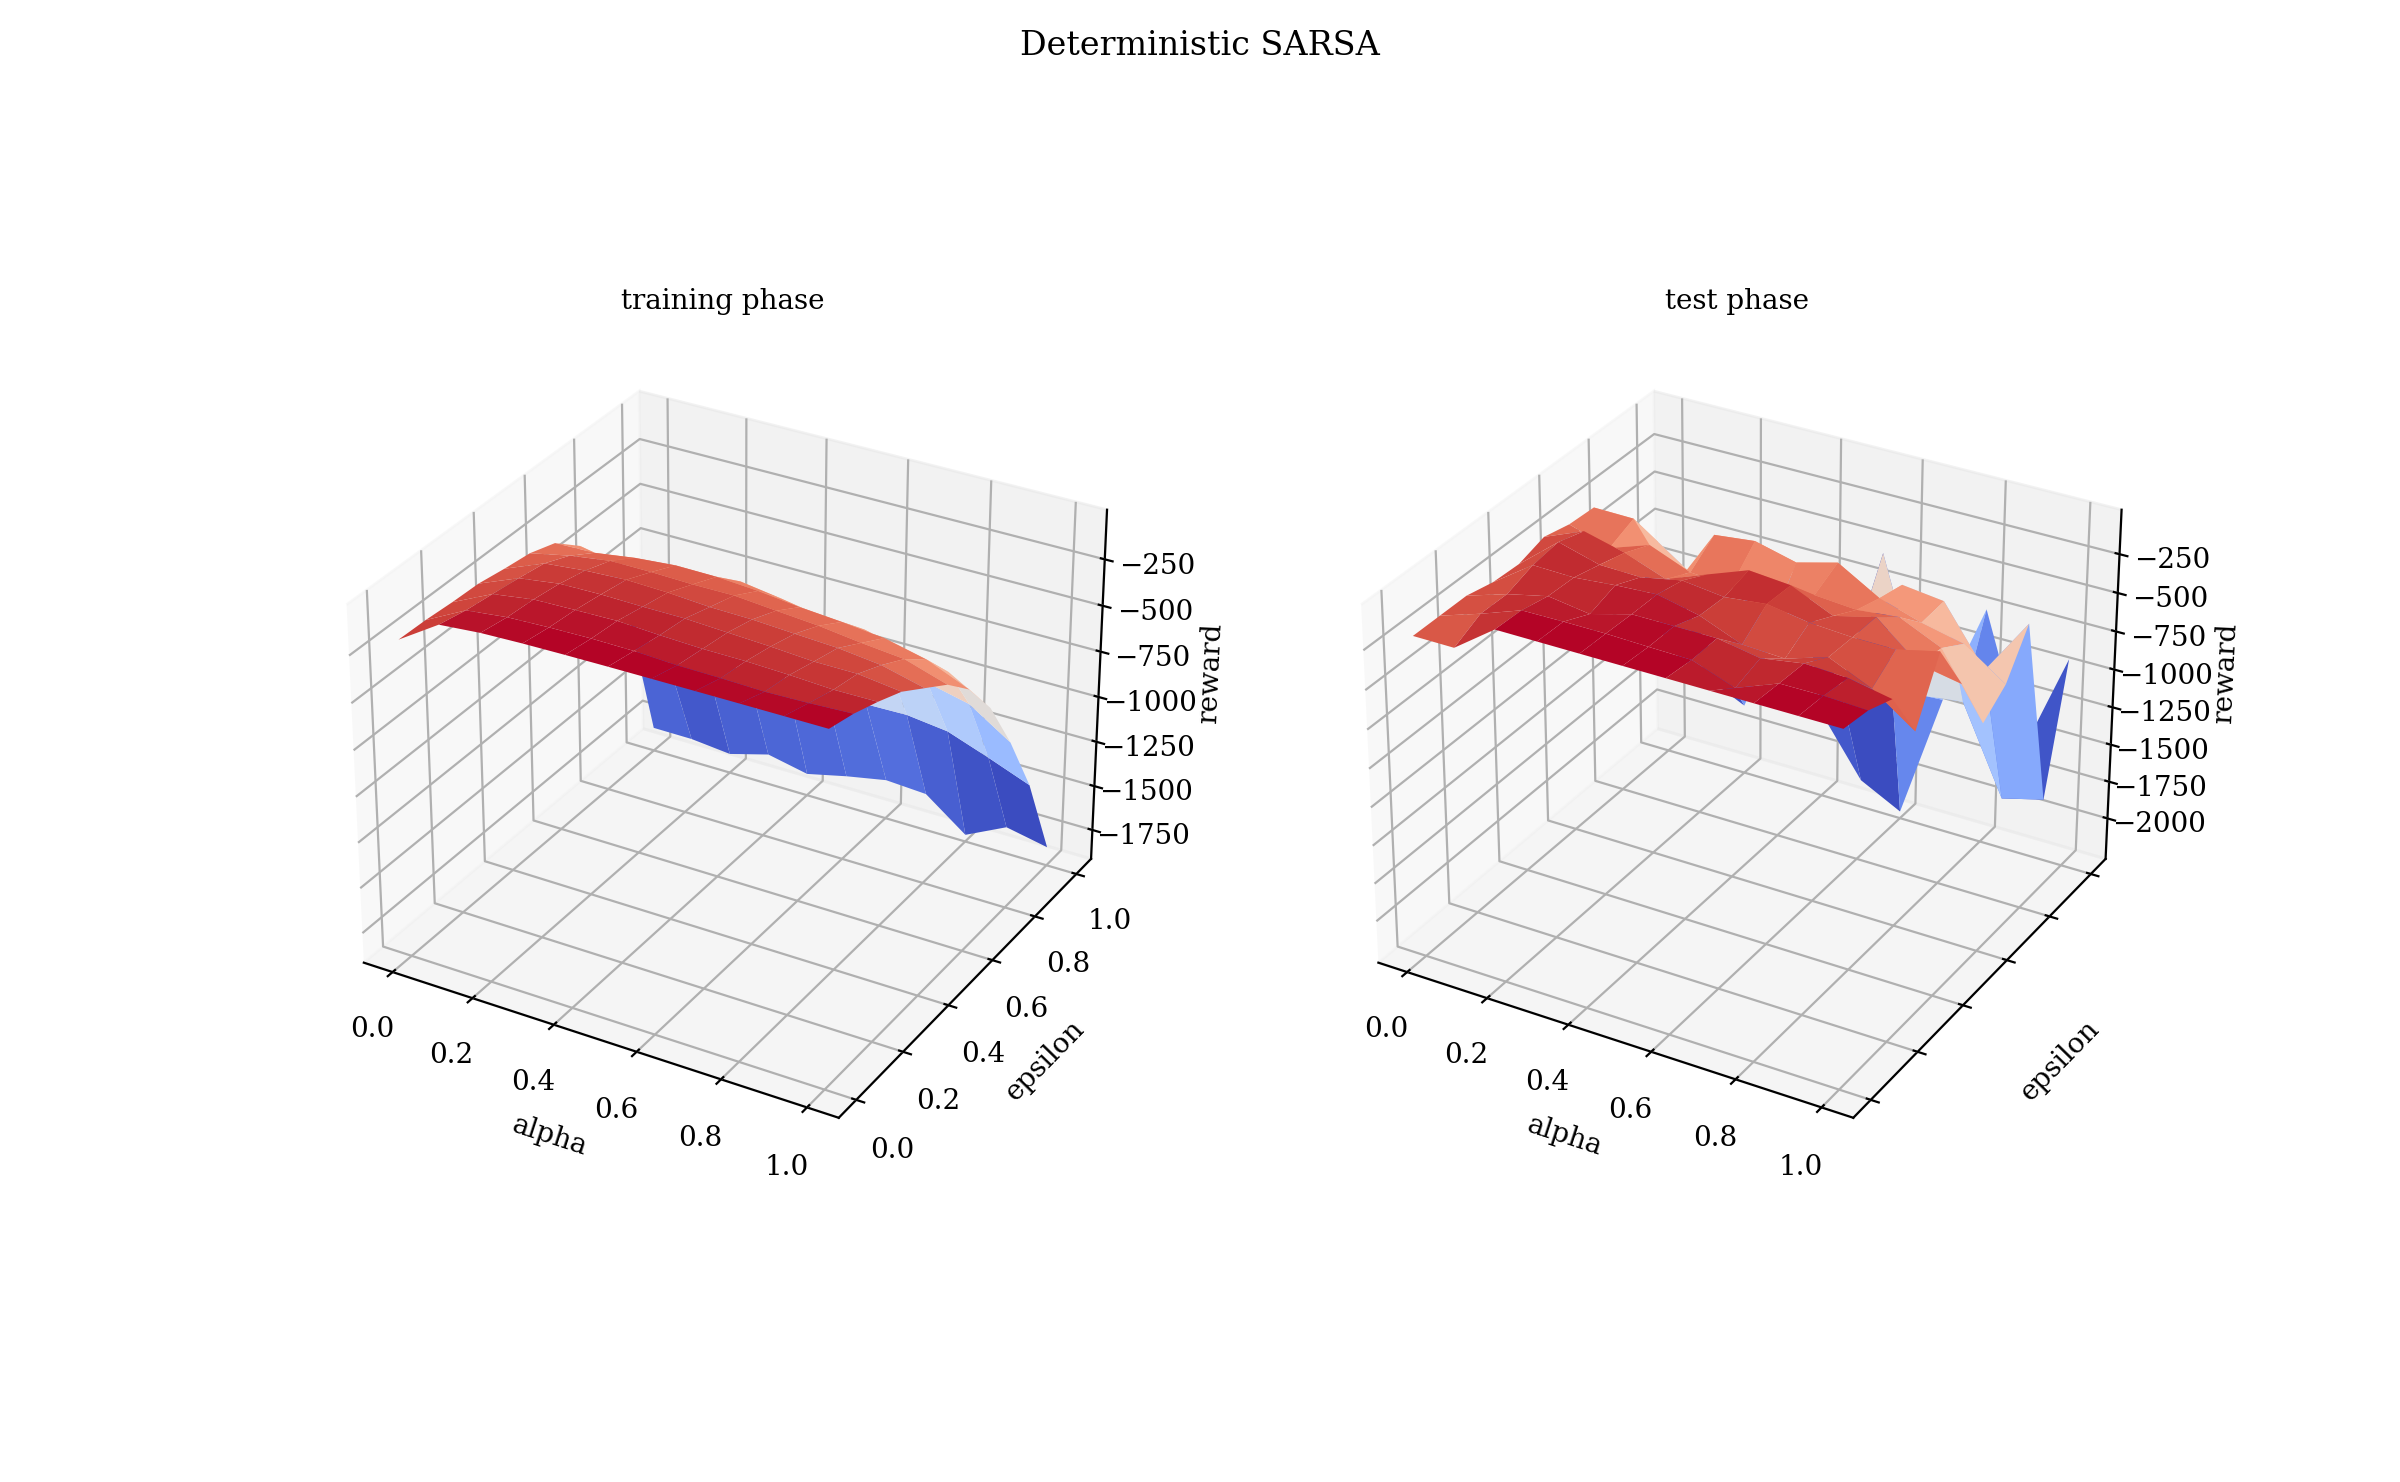
\includegraphics[width=1\linewidth]{../plots/det_sarsa_alpha_eps.png}  
    \caption{Training and test-reward for the deterministic SARSA model under $\epsilon$ and $\alpha$ sweeps}
    \label{fig:det_sarsa_alpha_eps}
\end{figure}



\begin{figure}[H]
    \centering
    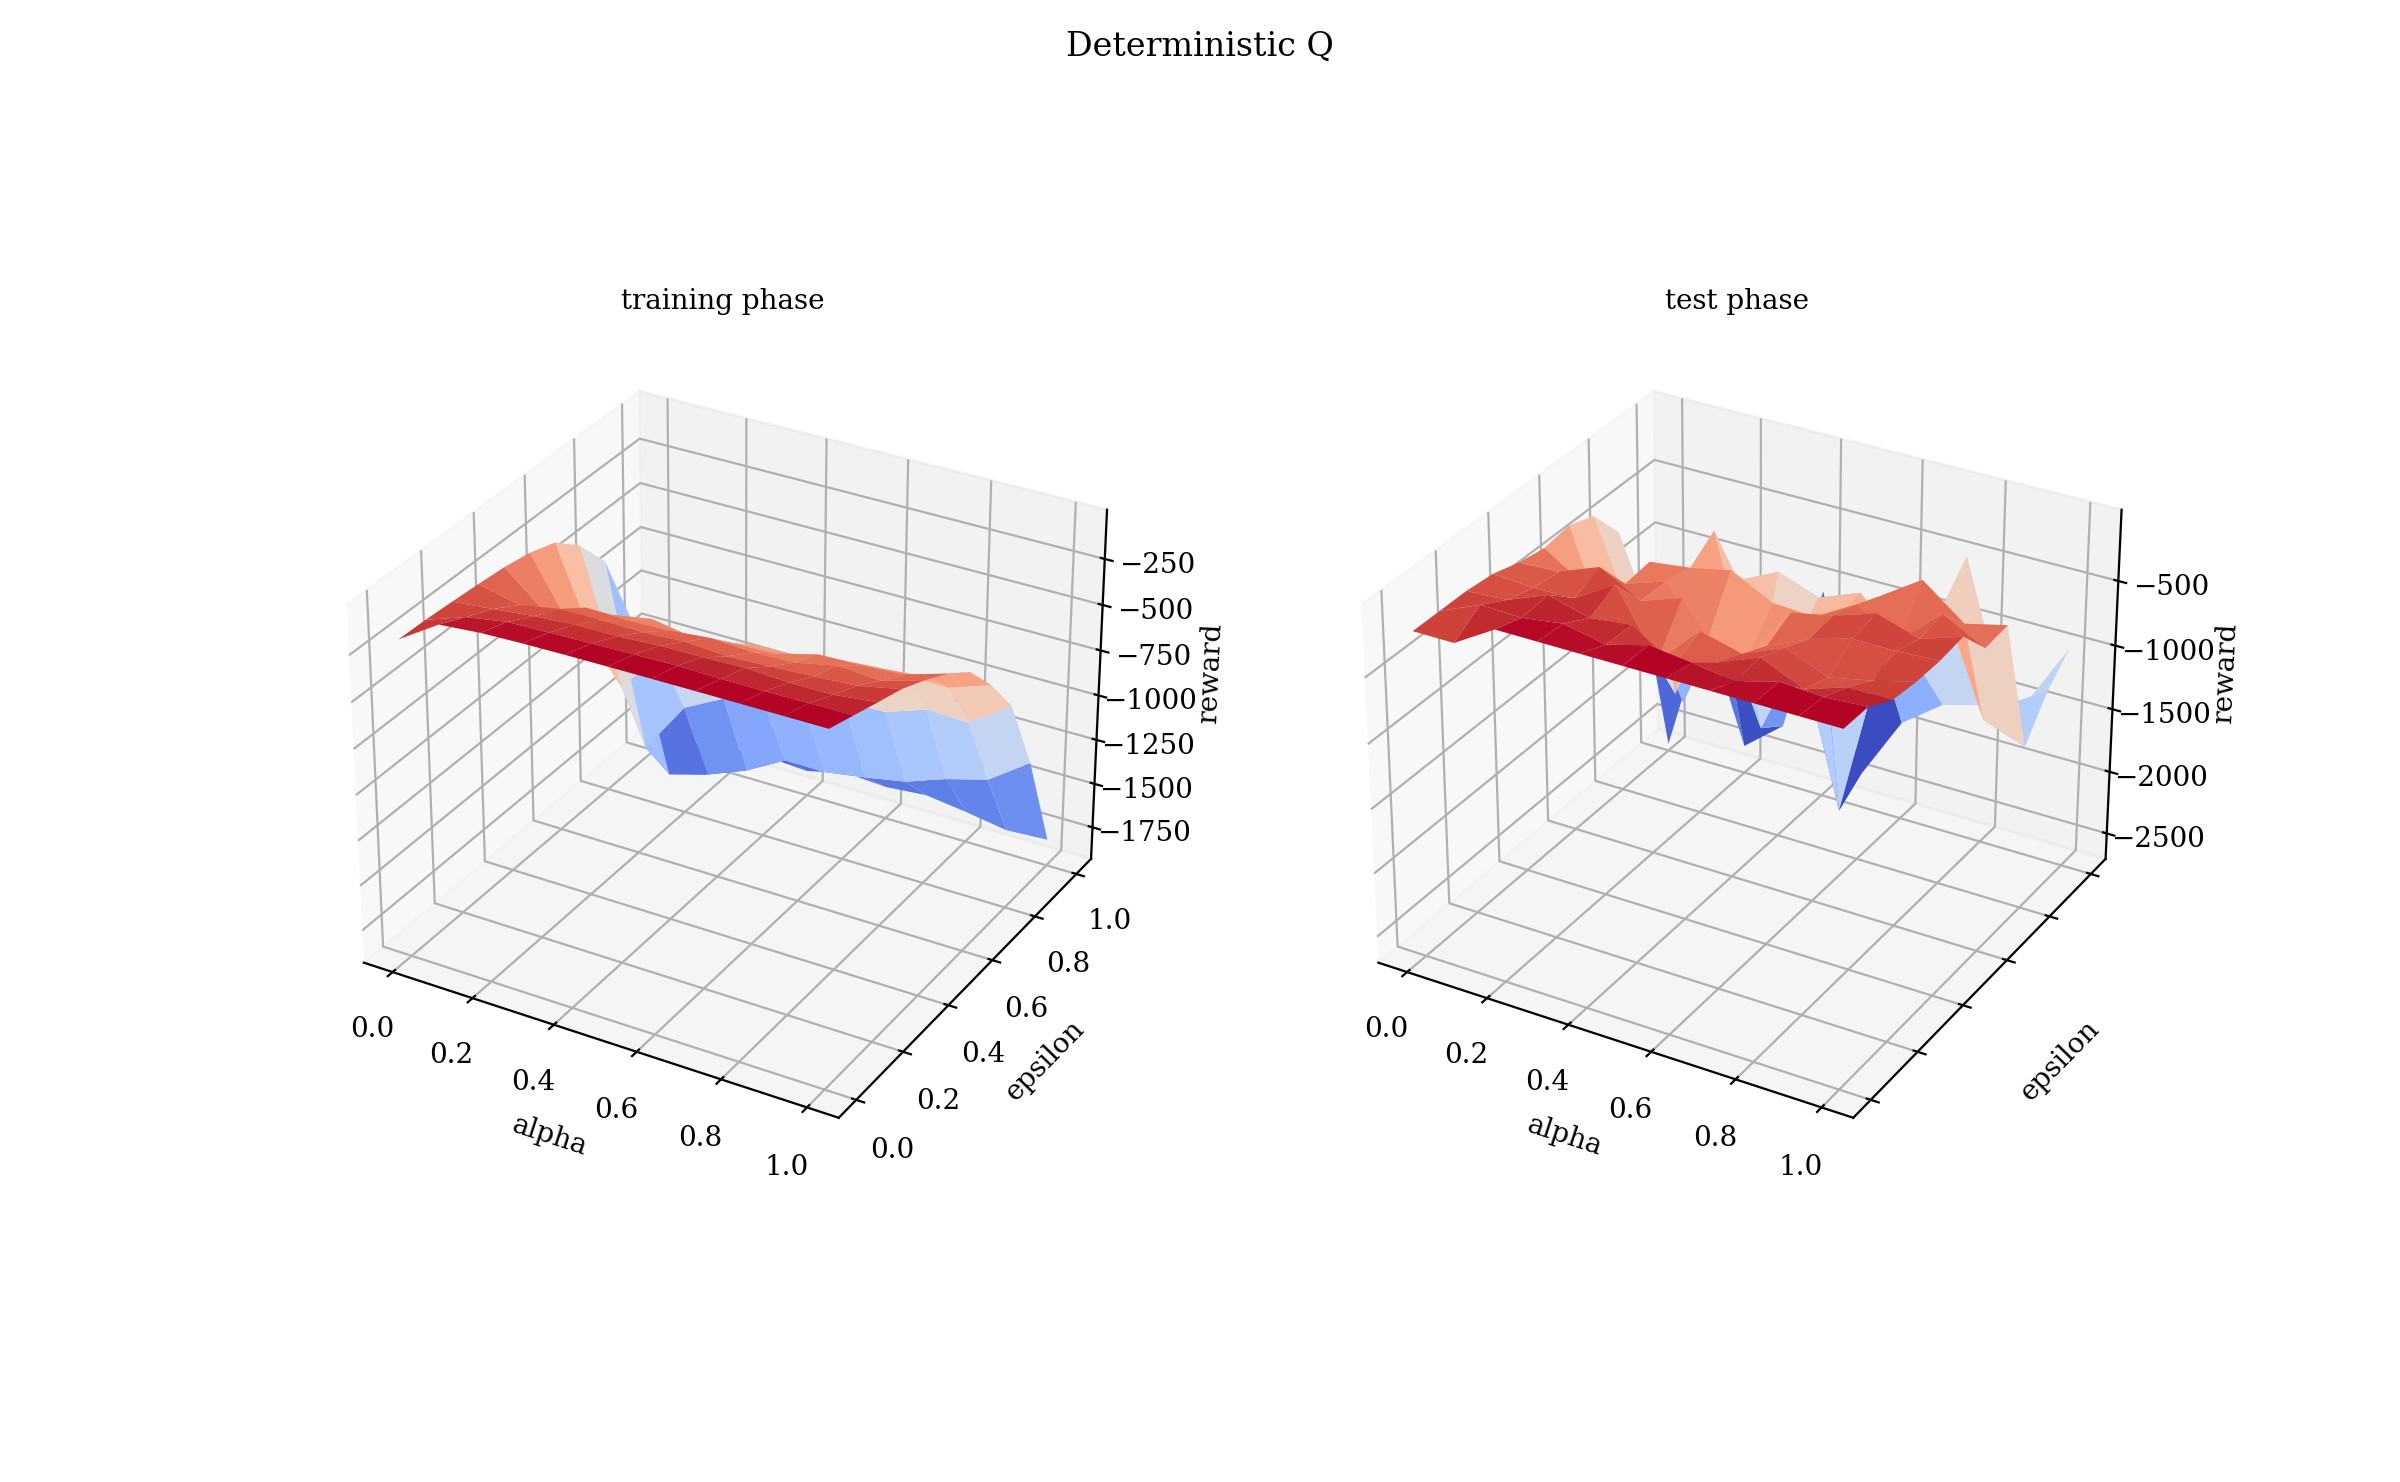
\includegraphics[width=1\linewidth]{../plots/det_Q_alpha_eps.png}  
    \caption{Training and test-reward for the deterministic Q-learning model under $\epsilon$ and $\alpha$ sweeps}
    \label{fig:det_Q_alpha_eps}
\end{figure}



\begin{figure}[H]
    \centering
    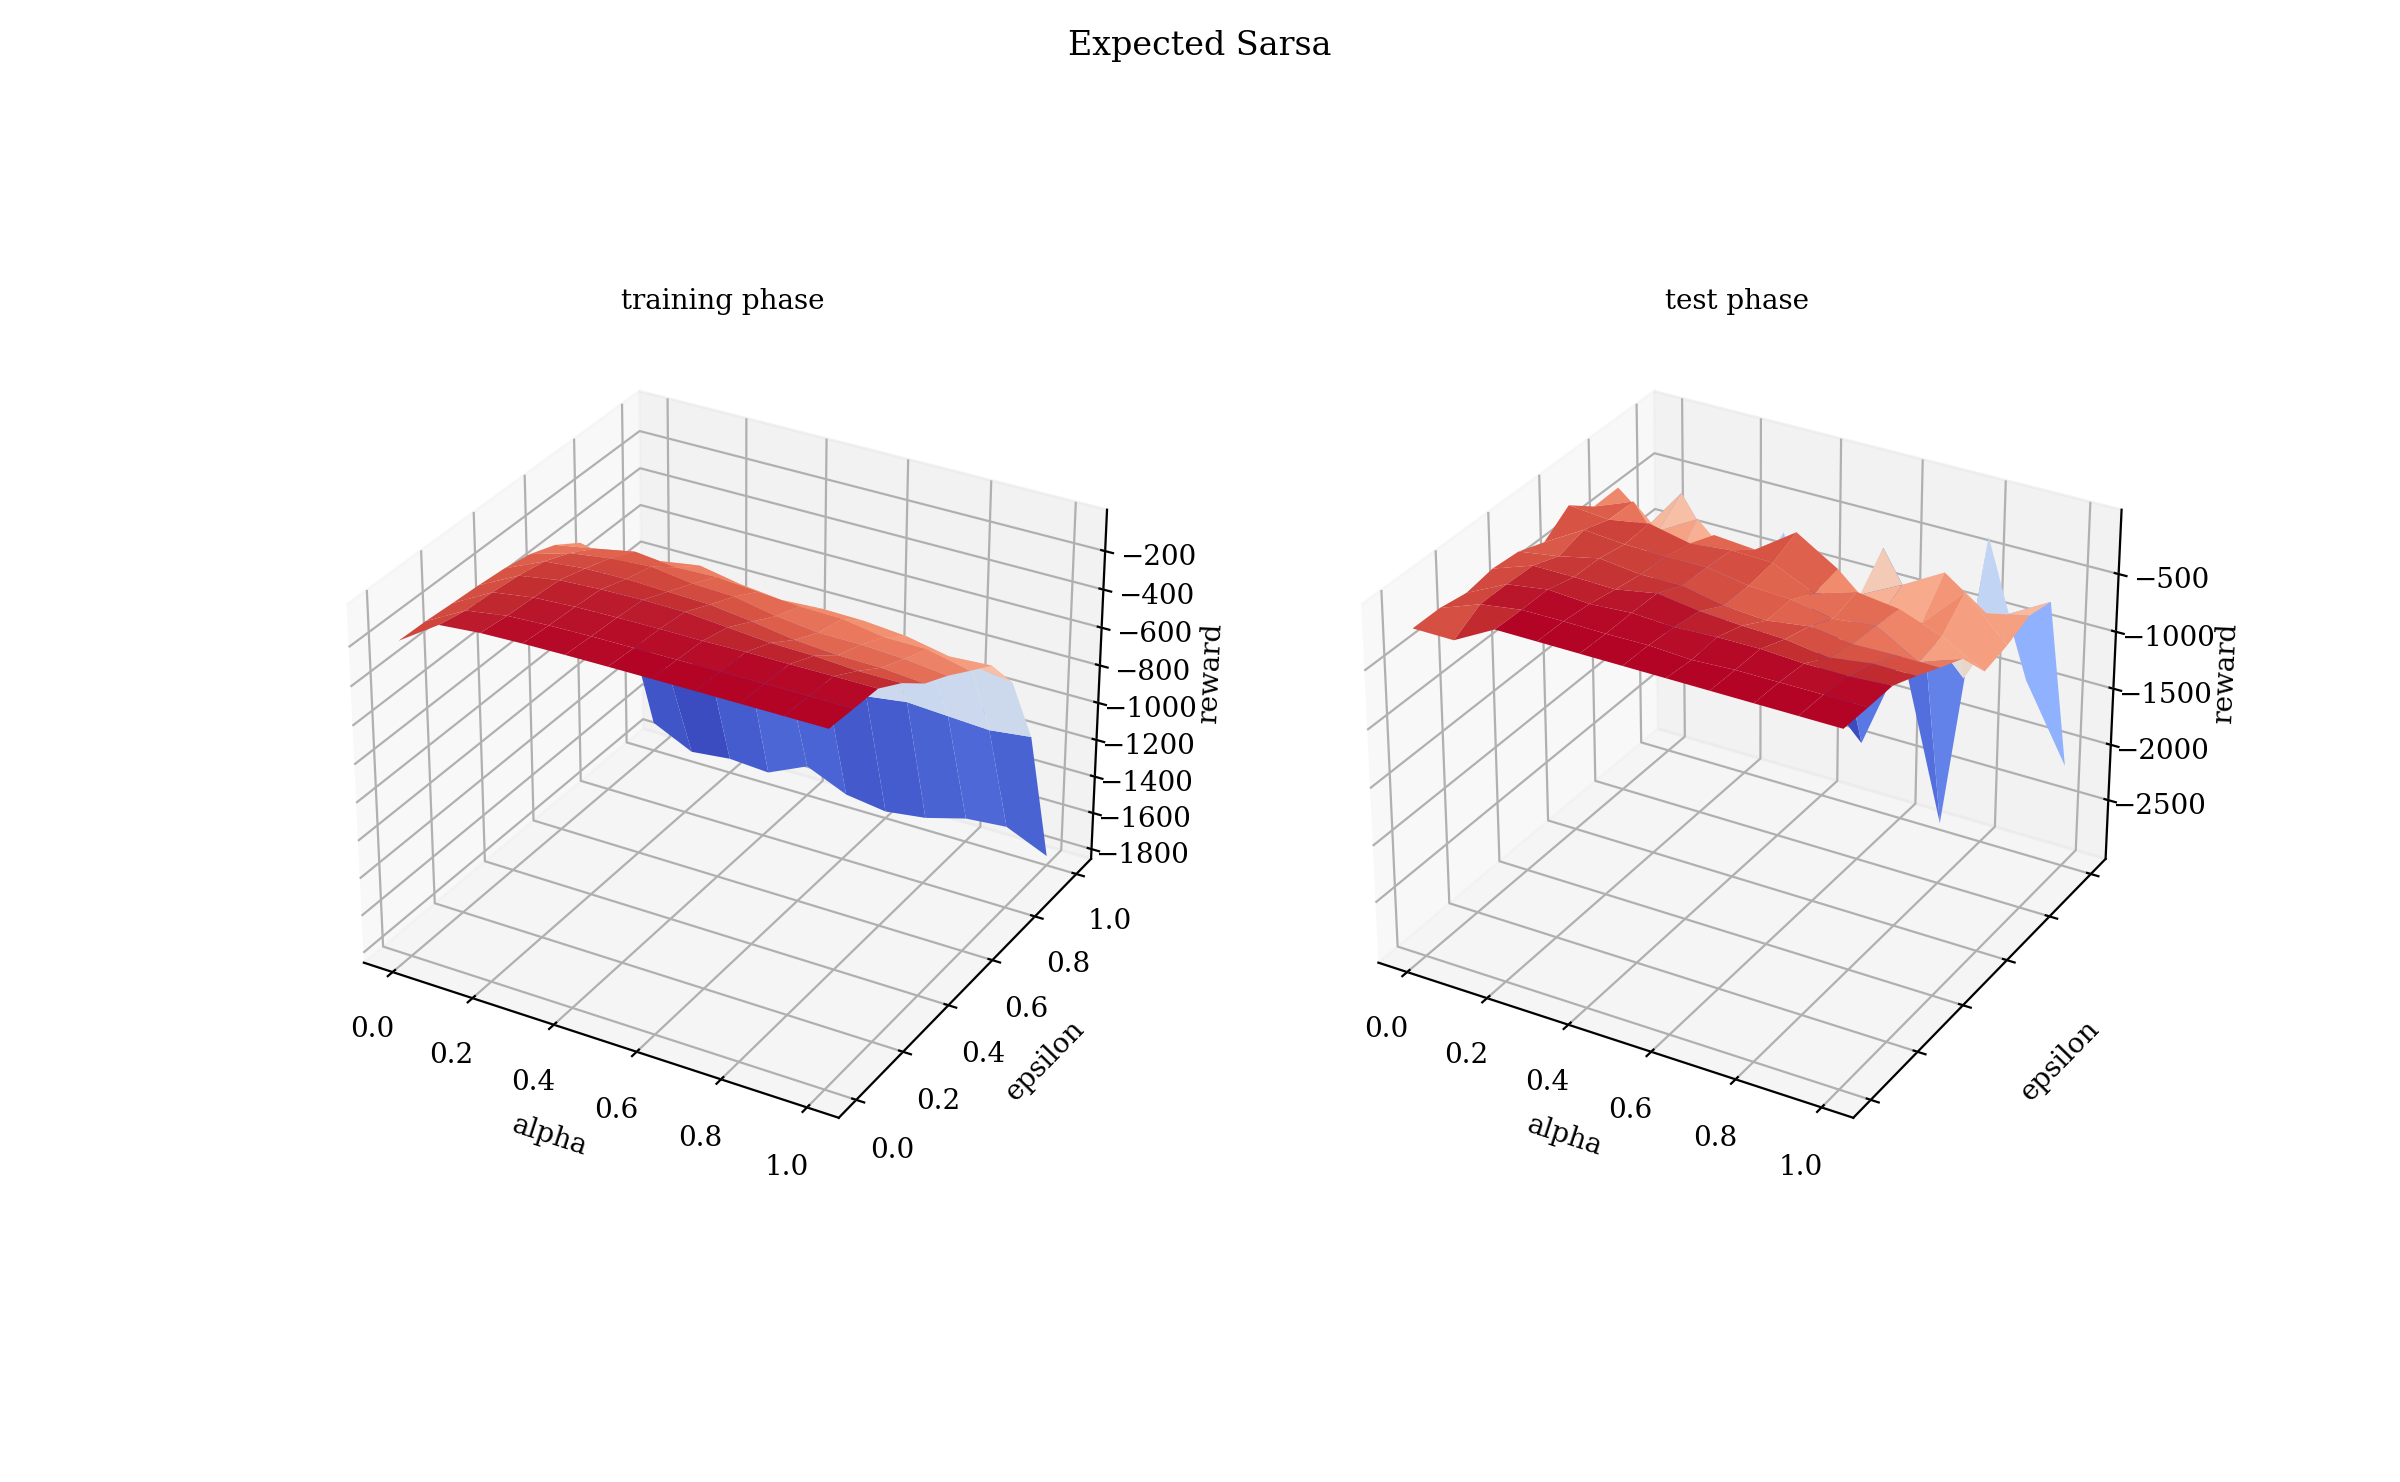
\includegraphics[width=1\linewidth]{../plots/expected_sarsa_alpha_eps.png}  
    \caption{Training and test-reward for the expected SARSA model under $\epsilon$ and $\alpha$ sweeps}
    \label{fig:expected_sarsa_alpha_eps}
\end{figure}

As we expect, we see the best test-performance for very low epsilon values, since the optimal policy is the greedy one, and not an epsilon-greedy policy that randomly chooses sub-optimal actions.
The deterministic SARSA algorithm was able to find the optimal solutions of the grid world problem with a accumulated return of -13, and achieved this with multiple parameter combinations during the test runs, but always with $\epsilon = 0$. The exact combinations and rewards can be found in Table \ref{table:deterministic_sarsa_results}.


\begin{table}[H]
\begin{centering}
	\begin{tabular}{ccccc}
	$\alpha$ & $\epsilon$ & $\gamma$ & reward &  \\
	0.6   & 0   & 0.9   & -13     &  \\
	0.2   & 0   & 0.9   & -13     &  \\
	0.8   & 0   & 0.9   & -13     & 
	\end{tabular}
    \caption{Overview of hyperparameter combinations with corresponding return for deterministic SARSA}
    \label{table:deterministic_sarsa_results}
\end{centering}
\end{table}

The deterministic Q-learning algorithm showed similar results. Againg, the algorithm found the optimal solution with multiple parameter sets, as shown in Table \ref{table:deterministic_Q_results}.

\begin{table}[H]
\begin{centering}
	\begin{tabular}{ccccc}
	$\alpha$ & $\epsilon$ & $\gamma$ & reward &  \\
	0.2   & 0   & 0.9   & -13     &  \\
	0.3   & 0   & 0.9   & -13     &  \\
	1     & 0   & 0.9   & -13     & 
	\end{tabular}
    \caption{Overview of hyperparameter combinations with corresponding return for deterministic Q-learning}
    \label{table:deterministic_Q_results}

\end{centering}
\end{table}

Likewise, the expected SARSA algorithm achieved the same results under multiple hyperparameter combinations, as shown in Table \ref{table:expected_sarsa_results}.


\begin{table}[H]
\begin{centering}
	\begin{tabular}{ccccc}
	$\alpha$ & $\epsilon$ & $\gamma$ & reward &  \\
	0.3   & 0   & 0.9   & -13     &  \\
	0.6   & 0   & 0.9   & -13     &  \\
	1     & 0   & 0.9   & -13     & 
	\end{tabular}
    \caption{Overview of hyperparameter combinations with corresponding return for expected SARSA}
    \label{table:expected_sarsa_results}
\end{centering}
\end{table}





\subsection{Comparing the influence of hyperparameter $\gamma$}
Similar to $\epsilon$, we made parameter sweeps with hyperparameter $\gamma$ in order to show its influence. It was again evaluated in the range 0..1 with a stepsize of 0.1, 11 different values in total, as was $\alpha$, giving a total of 121 combinations. $\epsilon$ was set to 0.1 for these runs. The training and test-performances for the parameter sweeps are shown in Figures \ref{fig:det_sarsa_alpha_gamma}, \ref{fig:det_Q_alpha_gamma} and \ref{fig:exp_sarsa_alpha_gamma}.
The training and test performances of deterministic Q-learning seem to be generally higher than for the other algorithms, and that over a wider range of parameter settings (Figure \ref{fig:det_Q_alpha_gamma}). The  expected SARSA algorithm appears to achieve similar performance, but only on a narrow range of $\gamma$ values (Figure \ref{fig:exp_sarsa_alpha_gamma}).


\begin{figure}[H]
    \centering
    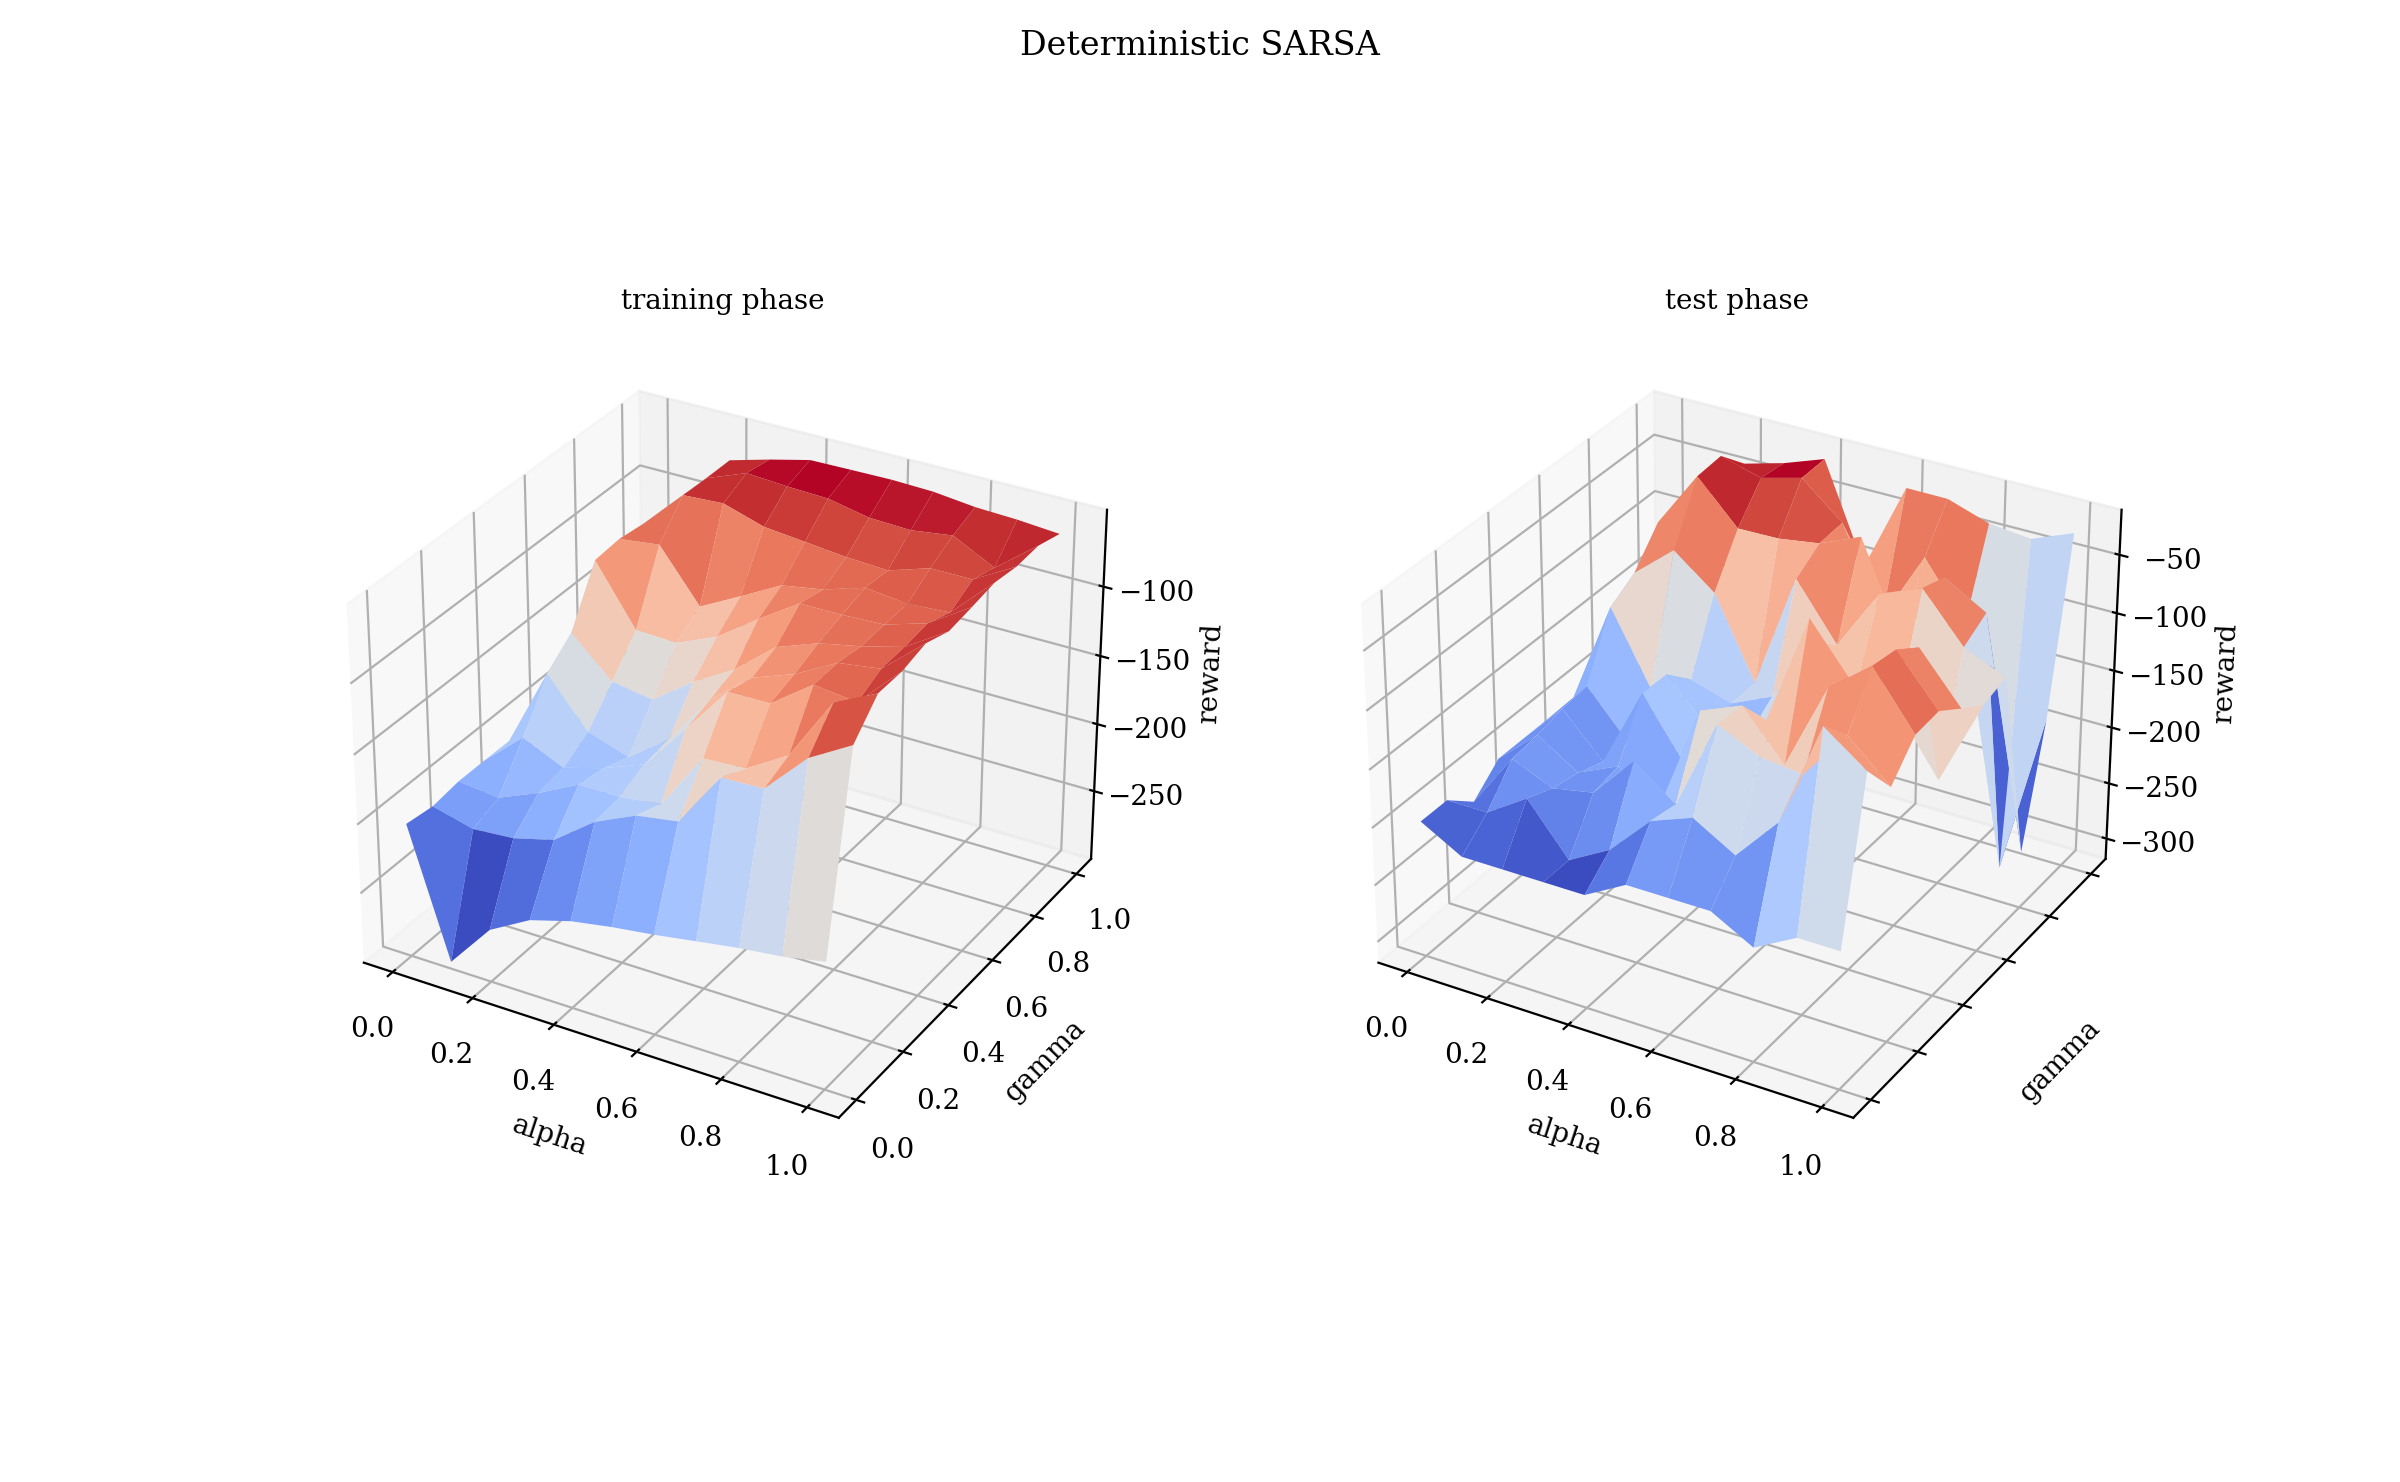
\includegraphics[width=1\linewidth]{../plots/det_sarsa_alpha_gamma.png}  
    \caption{Training and test-reward for the deterministic SARSA model under $\gamma$ and $\alpha$ sweeps}
    \label{fig:det_sarsa_alpha_gamma}
\end{figure}



\begin{figure}[H]
    \centering
    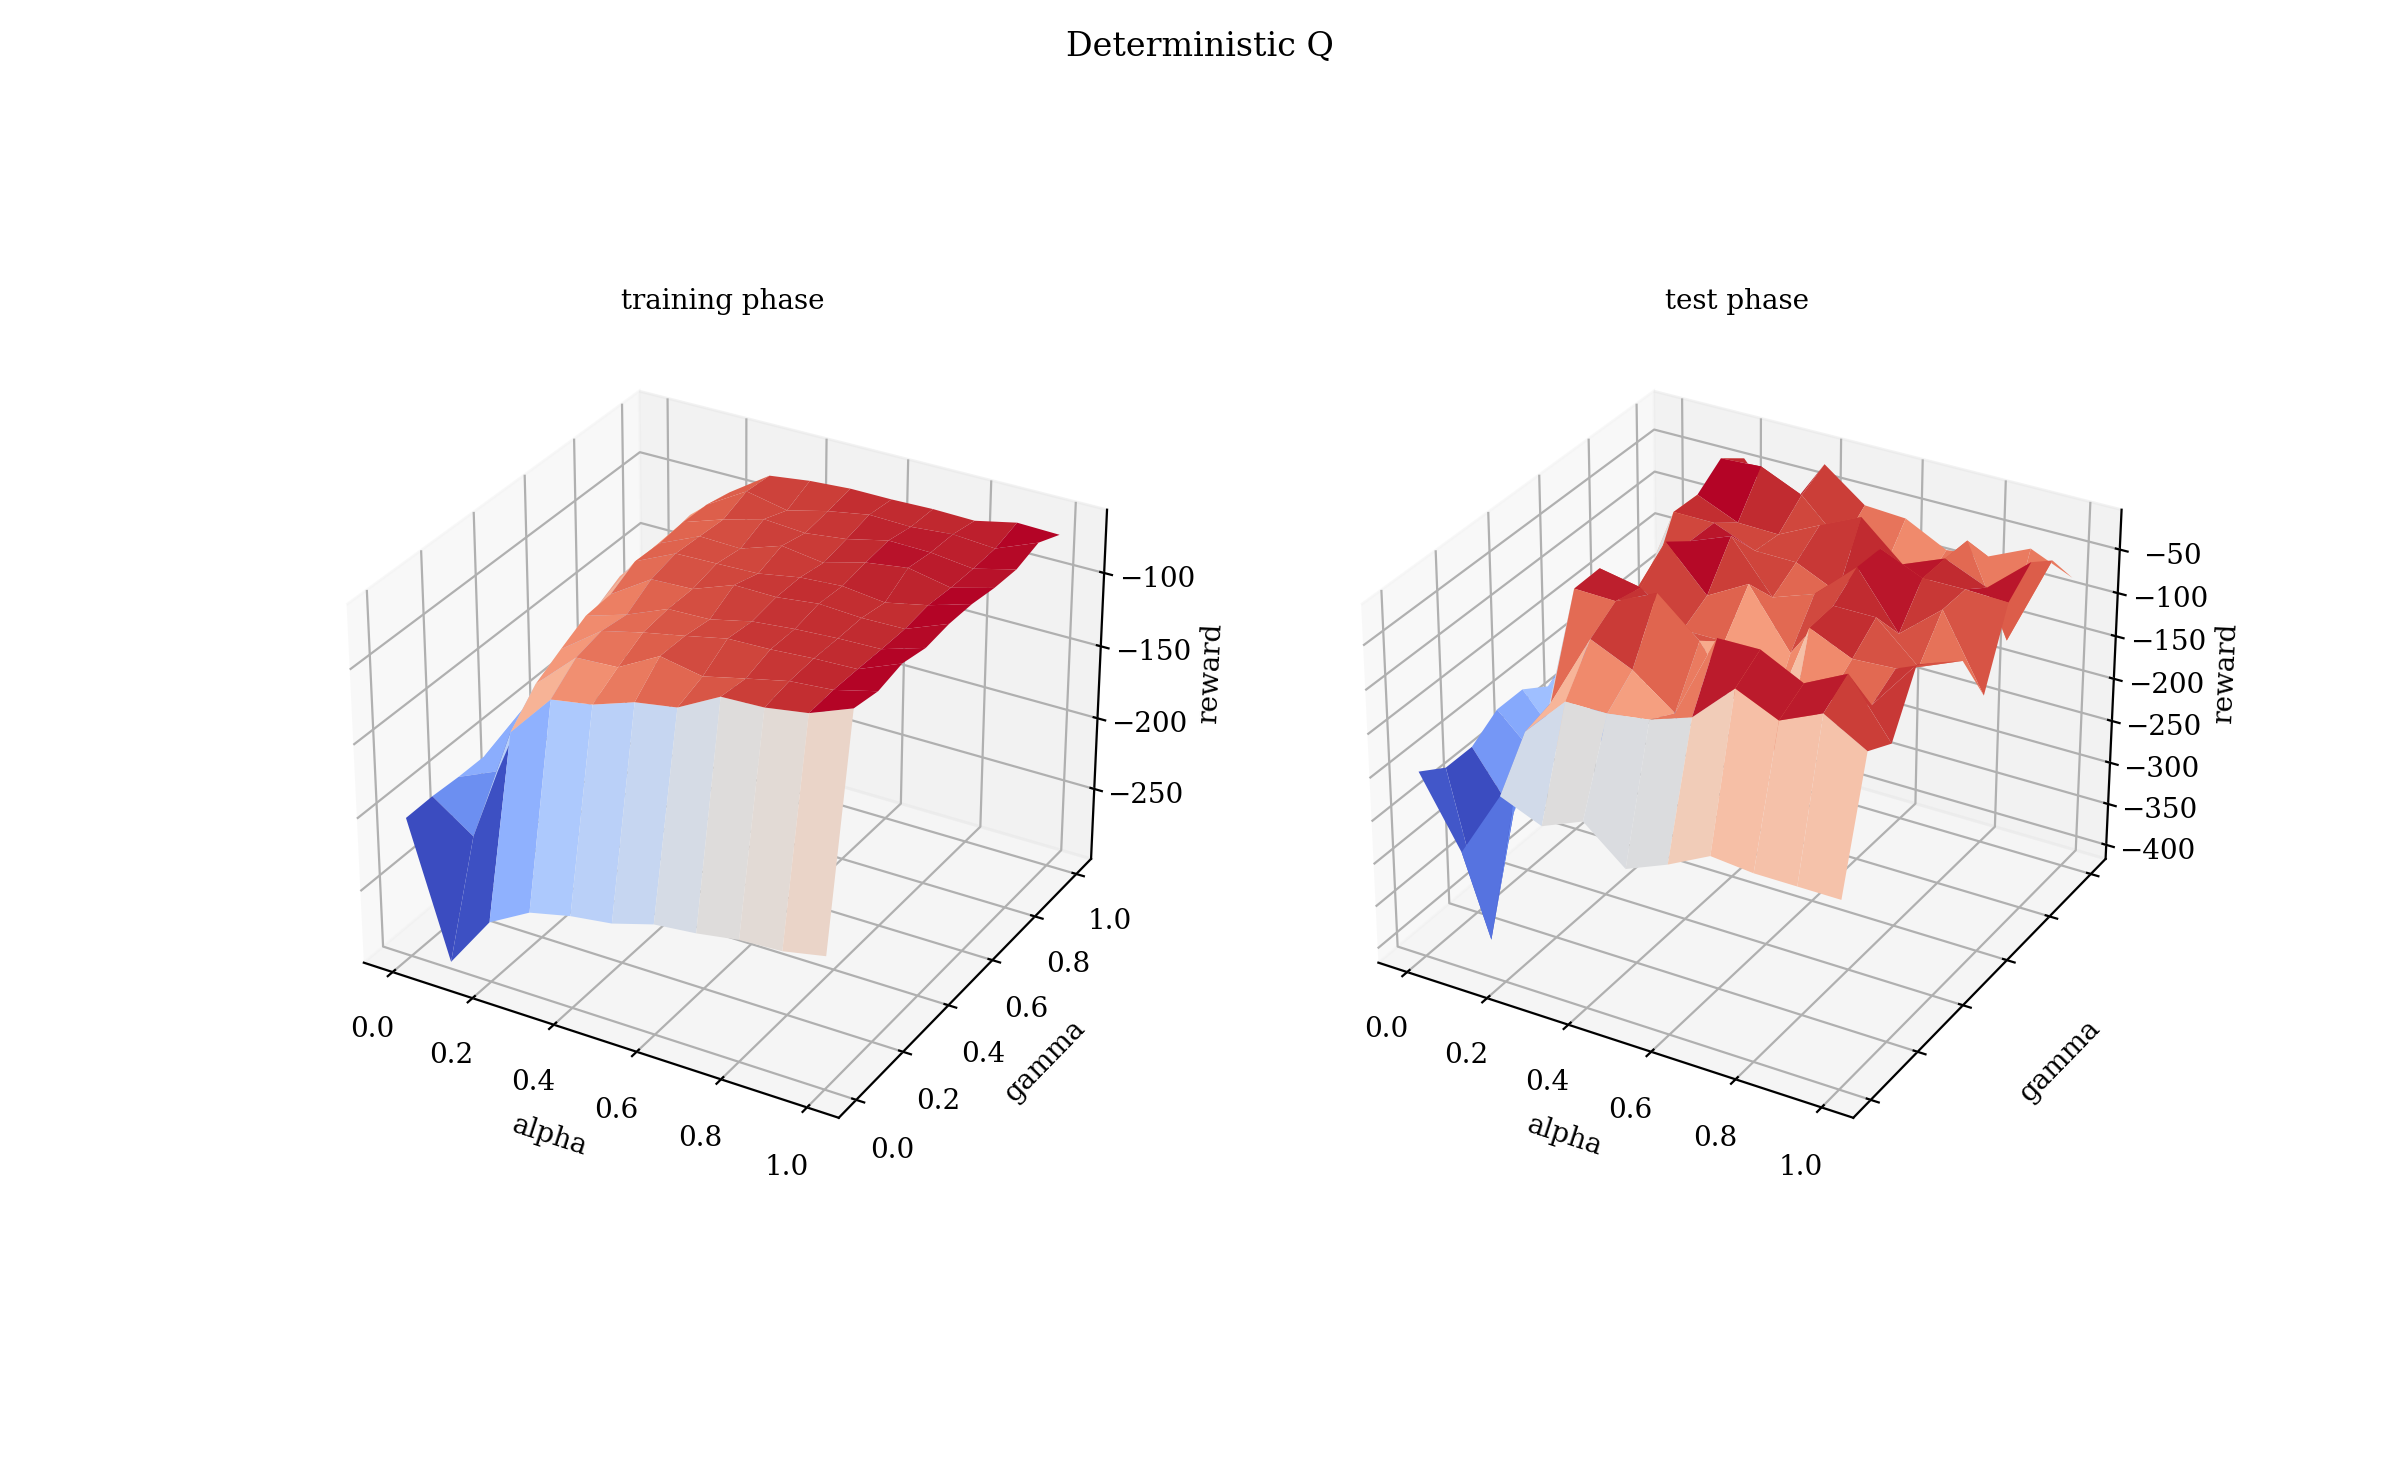
\includegraphics[width=1\linewidth]{../plots/det_Q_alpha_gamma.png}  
    \caption{Training and test-reward for the deterministic Q-learning model under $\gamma$ and $\alpha$ sweeps}
    \label{fig:det_Q_alpha_gamma}
\end{figure}




\begin{figure}[H]
    \centering
    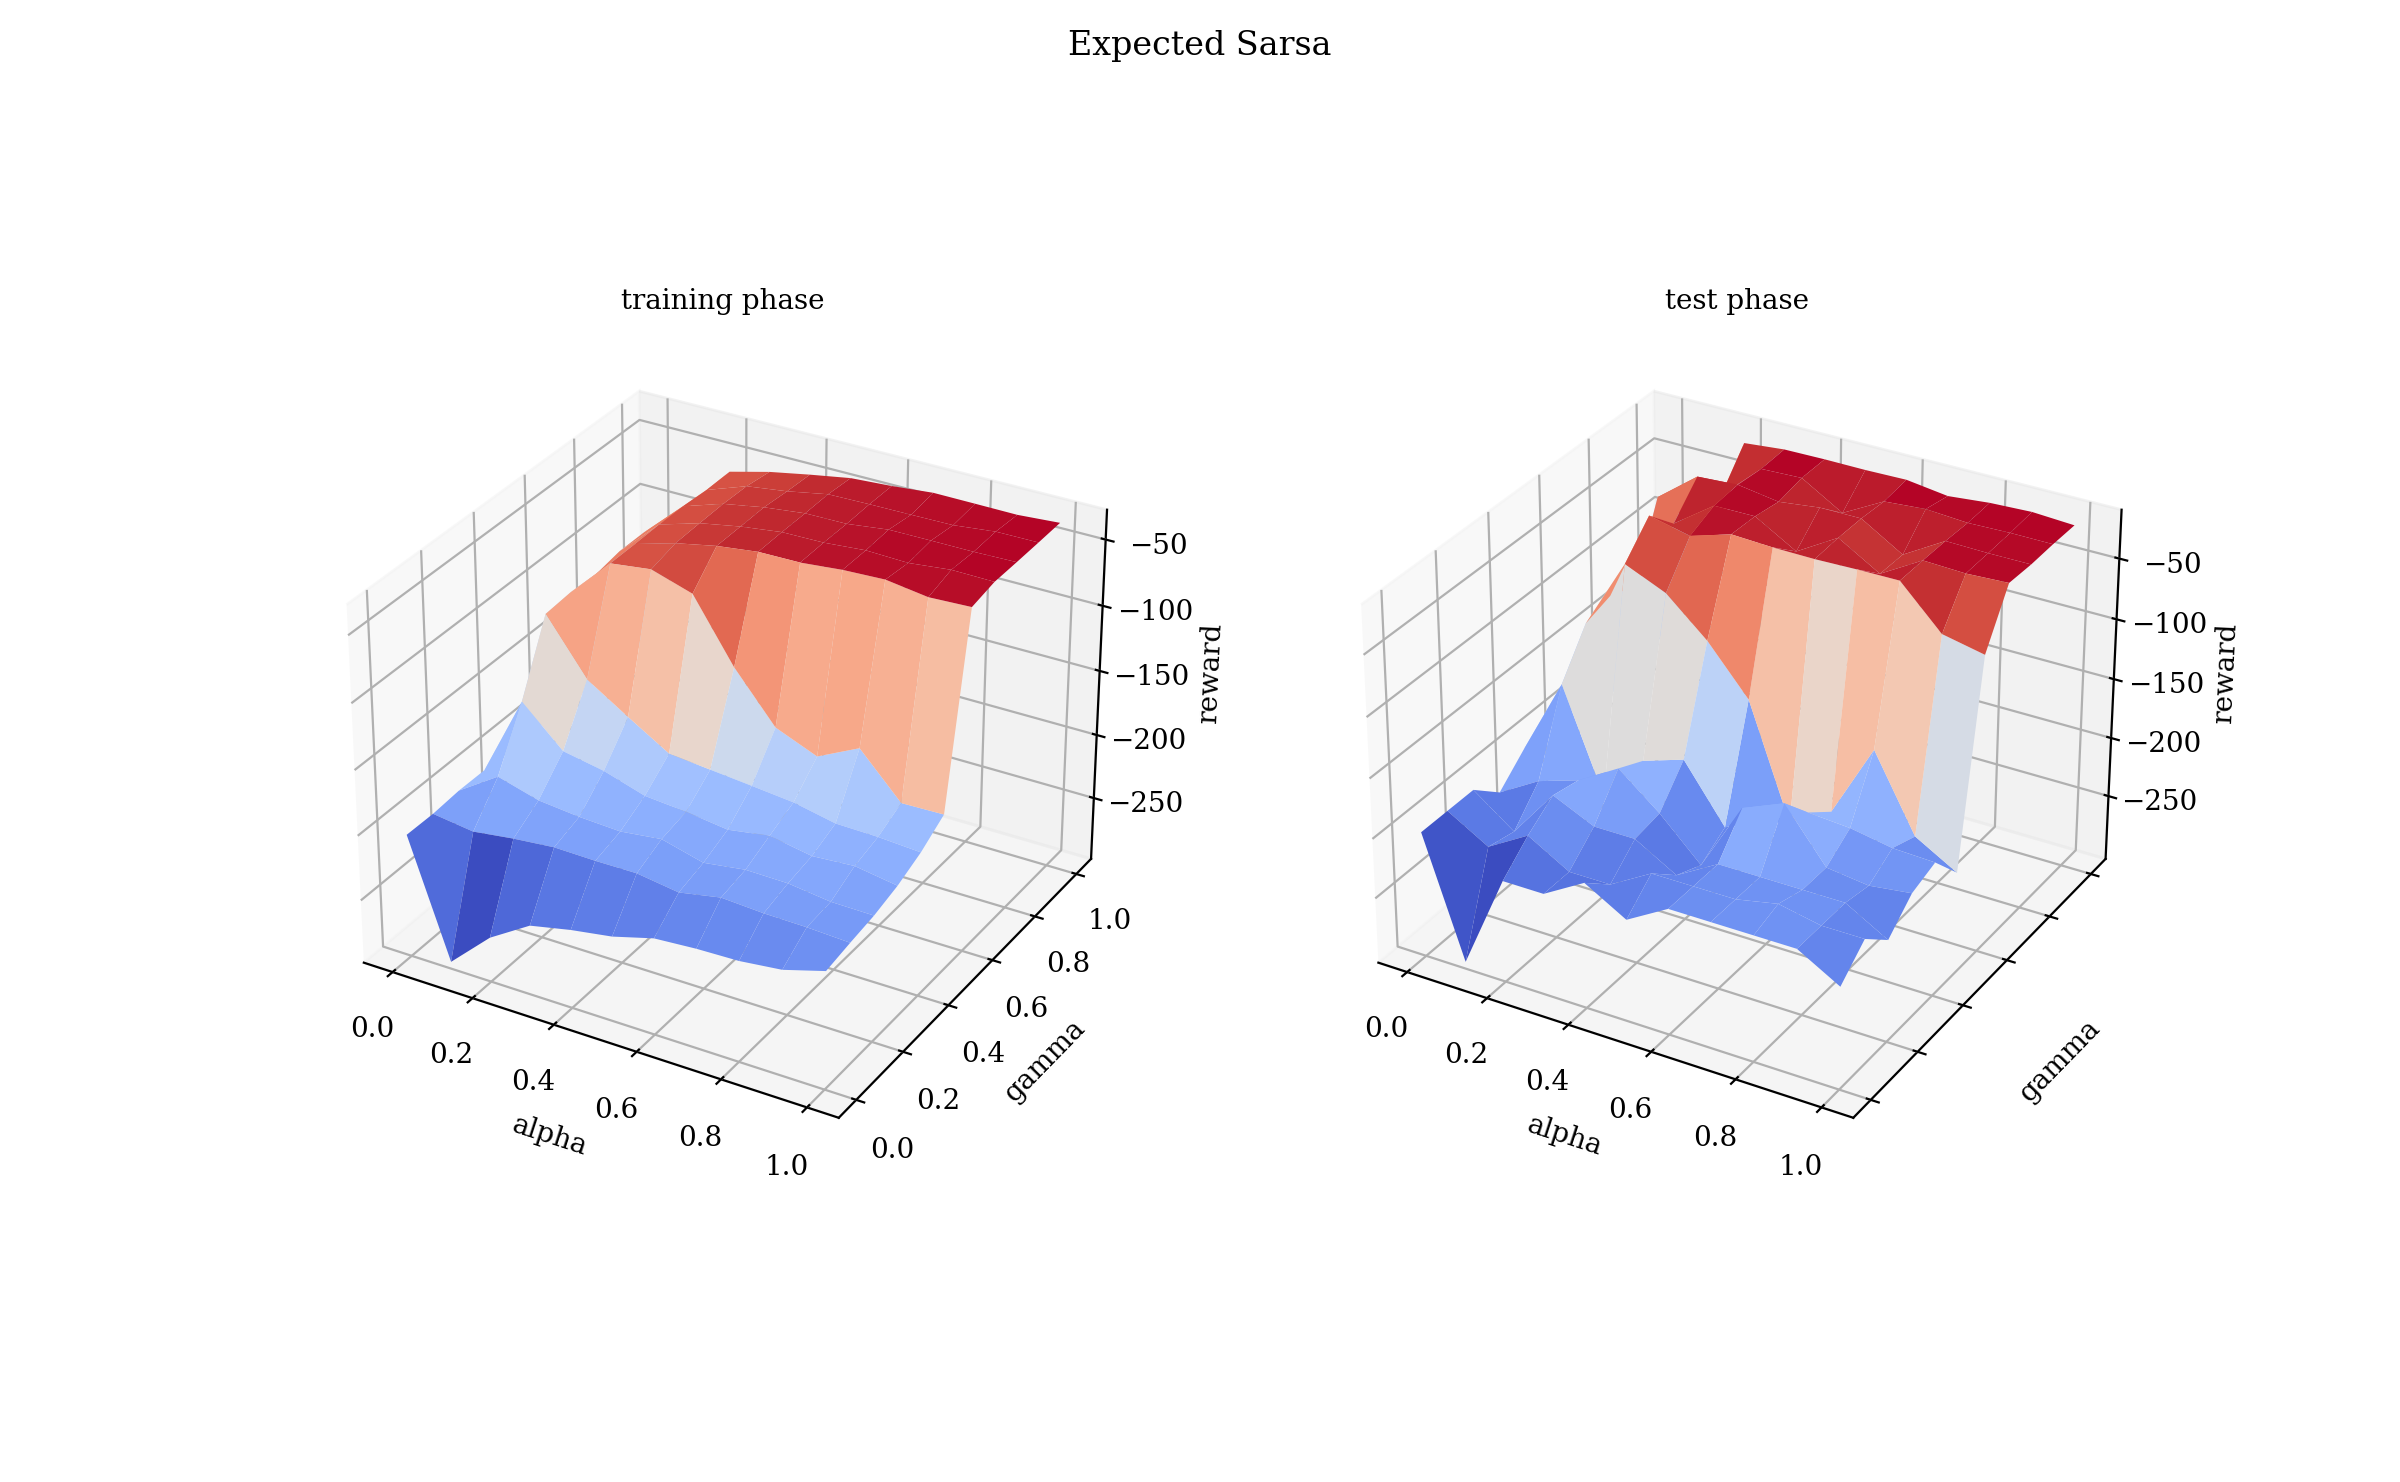
\includegraphics[width=1\linewidth]{../plots/expected_sarsa_alpha_gamma.png}  
    \caption{Training and test-reward for the expected SARSA model under $\gamma$ and $\alpha$ sweeps}
    \label{fig:exp_sarsa_alpha_gamma}
\end{figure}



The parameter sweeps for $\alpha$ and $\gamma$ made apparent that higher $\gamma$ values in the range of 0.8..1 are beneficial to the test performance. While the $\alpha - \epsilon$ sweeps did not exhibit a strong influence of $\alpha$, here we see a much stronger return for high values of $\alpha$ than for low values during the training runs. Over all algorithms, the best test performances were lower than during the $\alpha - \epsilon$ sweeps. This can be explained by the value of $\epsilon$ that was set to a fixed value of 0.1, hindering the algorithm from converging to the optimal policy. The best performing parameter sets for deterministic SARSA can be found in Table \ref{table:deterministic_sarsa_results_gamma_sweep}.


\begin{table}[H]
\begin{centering}
	\begin{tabular}{ccccc}
	$\alpha$ & $\epsilon$ & $\gamma$ & reward &  \\
	0.2   & 0.1   & 0.9   & -18.0     &  \\
	0.4   & 0.1   & 1.0   & -18.8     &  \\
	0.4   & 0.1   & 0.9   & -18.2     & 
	\end{tabular}
    \caption{Overview of hyperparameter combinations with corresponding return for deterministic SARSA 				under $\gamma$ and $\alpha$ sweeps}
    \label{table:deterministic_sarsa_results_gamma_sweep}
\end{centering}
\end{table}

The Q-learning algorithm performed better than the determistic SARSA algorithm in that it found optimal or almost optimal strategies with total rewards of -13 or -13.4 in three cases, as documented in Table \ref{table:deterministic_Q_results_gamma_sweep}.


\begin{table}[H]
\begin{centering}
	\begin{tabular}{ccccc}
	$\alpha$ & $\epsilon$ & $\gamma$ & reward &  \\
	0.7   & 0.1   & 0.6   & -13.4     &  \\
	0.6   & 0.1   & 0.8   & -13     &  \\
	0.3   & 0.1   & 0.9   & -13     & 
	\end{tabular}
    \caption{Overview of hyperparameter combinations with corresponding return for deterministic Q-learning under $\gamma$ and $\alpha$ sweeps}
    \label{table:deterministic_Q_results_gamma_sweep}
\end{centering}
\end{table}

Expected SARSA appeared to perform slightly better than deterministic SARSA, but not as good as Q-learning, and far from optimal. The best test results are shown in Table \ref{table:expected_sarsa_results_gamma_sweep}.

\begin{table}[H]
\begin{centering}
	\begin{tabular}{ccccc}
	$\alpha$ & $\epsilon$ & $\gamma$ & reward &  \\
	0.3   & 0.1   & 0.8   & -16.2     &  \\
	0.6   & 0.1   & 1.0   & -16.2     &  \\
	0.9   & 0.1   & 1.0   & -16.2     & 
	\end{tabular}
    \caption{Overview of hyperparameter combinations with corresponding return for expected SARSA 				under $\gamma$ and $\alpha$ sweeps}
    \label{table:expected_sarsa_results_gamma_sweep}
\end{centering}
\end{table}


\subsection{Why does $\gamma=1$ work in our MDP problems?}
Usually, $0 < \gamma < 1$ is required to ensure convergence of the value function for infinite episodes. Since our MDP problem is capped at 200 steps max, and the fact that a step into the cliff terminates the episode, infinite episode lengths are not possible. Therefore, the value function is bounded and the algorithm also work with $\gamma = 1$.